%==============================================================================
%  Mini project report
%  Bayesian Networks and Markov Models in Action, 2026--2027
%
%  Rules (see project/instructions.pdf):
%   - at most 8 single-column pages, excluding the references and the appendices;
%   - written in English; do not change the font size, the margins or the spacing;
%   - every number, figure and table must be produced by the submitted code.
%
%  Every table (tables/), figure (figures/) and number quoted in the text (numbers/, used as \val{key})
%  is written by the scripts in ../code/scripts (see ../code/README.md).
%==============================================================================
\documentclass[12pt]{article}

\usepackage[utf8]{inputenc}
\usepackage[T1]{fontenc}
\usepackage[english]{babel}
\usepackage{amsmath,amssymb,amsfonts}
\usepackage{graphicx}
\usepackage{booktabs}
\usepackage{xcolor}
\usepackage[ruled,vlined]{algorithm2e}
\usepackage[colorlinks=true,linkcolor=black,citecolor=blue,urlcolor=blue,breaklinks=true]{hyperref}

\usepackage{fancyhdr}
\pagestyle{fancy}

\usepackage[left=2.5cm,right=2.5cm,top=2.5cm,bottom=2.5cm]{geometry}
\setlength{\parskip}{6pt}

\usepackage[capitalise,noabbrev]{cleveref}

% Guidance text: delete every \guide{...} once the section is written.
\newcommand{\guide}[1]{\textit{\textcolor{gray}{#1}}}

% Notation used in the course (add your own macros here)
\newcommand{\E}{\mathbb{E}}
\newcommand{\by}{\mathbf{y}}
\newcommand{\given}{\,\vert\,}

% Our additions: a diagram package, a few macros, and the numbers written by the code
\usepackage{caption}
\captionsetup[table]{skip=6pt}  % space between a table caption and its table
\usepackage{tikz}
\usetikzlibrary{positioning,fit,arrows.meta}
\newcommand{\VaR}{\mathrm{VaR}}
\newcommand{\ES}{\mathrm{ES}}
\newcommand{\val}[1]{\ifcsname num@#1\endcsname\csname num@#1\endcsname\else\textbf{??#1??}\fi}
\expandafter\def\csname num@data-n-days\endcsname{5,031}
\expandafter\def\csname num@data-period\endcsname{03 Jan 2006 -- 31 Dec 2025}
\expandafter\def\csname num@data-mean\endcsname{0.042}
\expandafter\def\csname num@data-sd\endcsname{1.246}
\expandafter\def\csname num@data-worst\endcsname{-12.78}
\expandafter\def\csname num@data-best\endcsname{10.76}
\expandafter\def\csname num@data-beyond4-obs\endcsname{36}
\expandafter\def\csname num@data-beyond4-gauss\endcsname{0.32}
\expandafter\def\csname num@data-start-year\endcsname{2006}
\expandafter\def\csname num@data-end-year\endcsname{2025}
\expandafter\def\csname num@data-worst-date\endcsname{16 March 2020}
\expandafter\def\csname num@data-worst-loss\endcsname{12.78}

\expandafter\def\csname num@val-prior-dev\endcsname{2}
\expandafter\def\csname num@val-mu-true\endcsname{0.1}
\expandafter\def\csname num@val-sigma-true\endcsname{0.7}
\expandafter\def\csname num@val-mu-mean\endcsname{0.075}
\expandafter\def\csname num@val-mu-lo\endcsname{0.051}
\expandafter\def\csname num@val-mu-hi\endcsname{0.0993}
\expandafter\def\csname num@val-mu-mle\endcsname{0.076}
\expandafter\def\csname num@val-nu-true\endcsname{2.5}
\expandafter\def\csname num@val-nu-mean\endcsname{2.38}
\expandafter\def\csname num@val-nu-lo\endcsname{2.20}
\expandafter\def\csname num@val-nu-hi\endcsname{2.57}
\expandafter\def\csname num@val-acc-min\endcsname{0.32}
\expandafter\def\csname num@val-acc-max\endcsname{0.32}
\expandafter\def\csname num@val-rhat-max\endcsname{1.0005}
\expandafter\def\csname num@val-ess-min\endcsname{6,689}

\expandafter\def\csname num@cov-n-sets\endcsname{100}
\expandafter\def\csname num@cov-n-fits\endcsname{300}
\expandafter\def\csname num@cov-band-lo\endcsname{90}
\expandafter\def\csname num@cov-band-hi\endcsname{99}
\expandafter\def\csname num@cov-min\endcsname{90}
\expandafter\def\csname num@cov-max\endcsname{99}
\expandafter\def\csname num@cov-converged\endcsname{300}
\expandafter\def\csname num@cov-rhat-max\endcsname{1.0071}
\expandafter\def\csname num@cov-ess-min\endcsname{1,243}
\expandafter\def\csname num@cov-zmean-min\endcsname{-0.18}
\expandafter\def\csname num@cov-zmean-max\endcsname{0.21}
\expandafter\def\csname num@cov-zsd-min\endcsname{0.90}
\expandafter\def\csname num@cov-zsd-max\endcsname{1.18}
\expandafter\def\csname num@cov-nu4-z\endcsname{-0.17}
\expandafter\def\csname num@cov-fig-nu\endcsname{97}
\expandafter\def\csname num@cov-fig-var\endcsname{99}

\expandafter\def\csname num@fit-mu\endcsname{0.097}
\expandafter\def\csname num@fit-mu-lo\endcsname{0.073}
\expandafter\def\csname num@fit-mu-hi\endcsname{0.120}
\expandafter\def\csname num@fit-sigma\endcsname{0.683}
\expandafter\def\csname num@fit-nu\endcsname{2.48}
\expandafter\def\csname num@fit-nu-lo\endcsname{2.27}
\expandafter\def\csname num@fit-nu-hi\endcsname{2.71}
\expandafter\def\csname num@fit-sd\endcsname{1.58}
\expandafter\def\csname num@fit-sd-lo\endcsname{1.37}
\expandafter\def\csname num@fit-sd-hi\endcsname{1.92}
\expandafter\def\csname num@fit-g-mu\endcsname{0.041}
\expandafter\def\csname num@fit-g-s\endcsname{1.246}
\expandafter\def\csname num@fit-sample-sd\endcsname{1.246}
\expandafter\def\csname num@fit-n-draws\endcsname{72,000}
\expandafter\def\csname num@fit-nu-below4\endcsname{72,000}
\expandafter\def\csname num@fit-nu-below3\endcsname{71,997}
\expandafter\def\csname num@fit-nu-mle\endcsname{2.47}
\expandafter\def\csname num@fit-acc-t-min\endcsname{0.32}
\expandafter\def\csname num@fit-acc-t-max\endcsname{0.32}
\expandafter\def\csname num@fit-rhat-max\endcsname{1.0012}
\expandafter\def\csname num@fit-ess-min\endcsname{5,200}
\expandafter\def\csname num@fit-sd-ratio\endcsname{27}
\expandafter\def\csname num@cfg-seed\endcsname{2,026}
\expandafter\def\csname num@cfg-chains\endcsname{4}
\expandafter\def\csname num@cfg-start-spread\endcsname{5}
\expandafter\def\csname num@cfg-pilot-iter\endcsname{5,000}
\expandafter\def\csname num@cfg-pilot-rounds\endcsname{3}
\expandafter\def\csname num@cfg-n-iter\endcsname{20,000}
\expandafter\def\csname num@cfg-burn-in\endcsname{2,000}
\expandafter\def\csname num@cfg-kept\endcsname{18,000}
\expandafter\def\csname num@cov-cfg-pilot-iter\endcsname{2,000}
\expandafter\def\csname num@cov-cfg-n-iter\endcsname{6,000}
\expandafter\def\csname num@cov-cfg-burn-in\endcsname{1,000}

\expandafter\def\csname num@VaR97.5-g-plug\endcsname{2.40}
\expandafter\def\csname num@VaR97.5-g-pred\endcsname{2.40}
\expandafter\def\csname num@VaR97.5-g-lo\endcsname{2.34}
\expandafter\def\csname num@VaR97.5-g-hi\endcsname{2.46}
\expandafter\def\csname num@ES97.5-g-plug\endcsname{2.87}
\expandafter\def\csname num@ES97.5-g-pred\endcsname{2.87}
\expandafter\def\csname num@ES97.5-g-lo\endcsname{2.81}
\expandafter\def\csname num@ES97.5-g-hi\endcsname{2.94}
\expandafter\def\csname num@VaR99-g-plug\endcsname{2.86}
\expandafter\def\csname num@VaR99-g-pred\endcsname{2.86}
\expandafter\def\csname num@VaR99-g-lo\endcsname{2.79}
\expandafter\def\csname num@VaR99-g-hi\endcsname{2.93}
\expandafter\def\csname num@ES99-g-plug\endcsname{3.28}
\expandafter\def\csname num@ES99-g-pred\endcsname{3.28}
\expandafter\def\csname num@ES99-g-lo\endcsname{3.21}
\expandafter\def\csname num@ES99-g-hi\endcsname{3.35}
\expandafter\def\csname num@VaR99.9-g-plug\endcsname{3.81}
\expandafter\def\csname num@VaR99.9-g-pred\endcsname{3.81}
\expandafter\def\csname num@VaR99.9-g-lo\endcsname{3.73}
\expandafter\def\csname num@VaR99.9-g-hi\endcsname{3.89}
\expandafter\def\csname num@ES99.9-g-plug\endcsname{4.16}
\expandafter\def\csname num@ES99.9-g-pred\endcsname{4.16}
\expandafter\def\csname num@ES99.9-g-lo\endcsname{4.07}
\expandafter\def\csname num@ES99.9-g-hi\endcsname{4.25}
\expandafter\def\csname num@VaR97.5-t-plug\endcsname{2.36}
\expandafter\def\csname num@VaR97.5-t-pred\endcsname{2.36}
\expandafter\def\csname num@VaR97.5-t-lo\endcsname{2.25}
\expandafter\def\csname num@VaR97.5-t-hi\endcsname{2.48}
\expandafter\def\csname num@ES97.5-t-plug\endcsname{4.18}
\expandafter\def\csname num@ES97.5-t-pred\endcsname{4.20}
\expandafter\def\csname num@ES97.5-t-lo\endcsname{3.84}
\expandafter\def\csname num@ES97.5-t-hi\endcsname{4.64}
\expandafter\def\csname num@VaR99-t-plug\endcsname{3.59}
\expandafter\def\csname num@VaR99-t-pred\endcsname{3.60}
\expandafter\def\csname num@VaR99-t-lo\endcsname{3.36}
\expandafter\def\csname num@VaR99-t-hi\endcsname{3.87}
\expandafter\def\csname num@ES99-t-plug\endcsname{6.19}
\expandafter\def\csname num@ES99-t-pred\endcsname{6.23}
\expandafter\def\csname num@ES99-t-lo\endcsname{5.53}
\expandafter\def\csname num@ES99-t-hi\endcsname{7.07}
\expandafter\def\csname num@VaR99.9-t-plug\endcsname{9.48}
\expandafter\def\csname num@VaR99.9-t-pred\endcsname{9.55}
\expandafter\def\csname num@VaR99.9-t-lo\endcsname{8.31}
\expandafter\def\csname num@VaR99.9-t-hi\endcsname{11.02}
\expandafter\def\csname num@ES99.9-t-plug\endcsname{16.00}
\expandafter\def\csname num@ES99.9-t-pred\endcsname{16.23}
\expandafter\def\csname num@ES99.9-t-lo\endcsname{13.29}
\expandafter\def\csname num@ES99.9-t-hi\endcsname{19.77}
\expandafter\def\csname num@VaR97.5-hist\endcsname{2.62}
\expandafter\def\csname num@ES97.5-hist\endcsname{4.00}
\expandafter\def\csname num@VaR99-hist\endcsname{3.60}
\expandafter\def\csname num@ES99-hist\endcsname{5.39}
\expandafter\def\csname num@VaR99.9-hist\endcsname{8.09}
\expandafter\def\csname num@ES99.9-hist\endcsname{9.70}
\expandafter\def\csname num@VaR97.5-tails\endcsname{$-$2}
\expandafter\def\csname num@VaR97.5-param\endcsname{0.2}
\expandafter\def\csname num@VaR97.5-under\endcsname{-2}
\expandafter\def\csname num@VaR97.5-ratio\endcsname{1.0}
\expandafter\def\csname num@VaR99-tails\endcsname{26}
\expandafter\def\csname num@VaR99-param\endcsname{0.2}
\expandafter\def\csname num@VaR99-under\endcsname{21}
\expandafter\def\csname num@VaR99-ratio\endcsname{1.3}
\expandafter\def\csname num@VaR99.9-tails\endcsname{149}
\expandafter\def\csname num@VaR99.9-param\endcsname{0.7}
\expandafter\def\csname num@VaR99.9-under\endcsname{60}
\expandafter\def\csname num@VaR99.9-ratio\endcsname{2.5}
\expandafter\def\csname num@ES97.5-tails\endcsname{46}
\expandafter\def\csname num@ES97.5-param\endcsname{0.5}
\expandafter\def\csname num@ES97.5-under\endcsname{32}
\expandafter\def\csname num@ES97.5-ratio\endcsname{1.5}
\expandafter\def\csname num@ES99-tails\endcsname{89}
\expandafter\def\csname num@ES99-param\endcsname{0.7}
\expandafter\def\csname num@ES99-under\endcsname{47}
\expandafter\def\csname num@ES99-ratio\endcsname{1.9}
\expandafter\def\csname num@ES99.9-tails\endcsname{285}
\expandafter\def\csname num@ES99.9-param\endcsname{1.5}
\expandafter\def\csname num@ES99.9-under\endcsname{74}
\expandafter\def\csname num@ES99.9-ratio\endcsname{3.9}
\expandafter\def\csname num@risk-mcse-max\endcsname{0.08}
\expandafter\def\csname num@risk-n-batches\endcsname{10}

\expandafter\def\csname num@ppc-worst-obs\endcsname{-12.8}
\expandafter\def\csname num@ppc-q01-obs\endcsname{-3.6}
\expandafter\def\csname num@ppc-days-loss-obs\endcsname{21}
\expandafter\def\csname num@ppc-sd-obs\endcsname{1.25}
\expandafter\def\csname num@ppc-asym-obs\endcsname{-0.375}
\expandafter\def\csname num@ppc-acf-obs\endcsname{0.305}
\expandafter\def\csname num@ppc-worst-g-p\endcsname{1.00}
\expandafter\def\csname num@ppc-q01-g-p\endcsname{1.00}
\expandafter\def\csname num@ppc-days-loss-g-p\endcsname{0.00}
\expandafter\def\csname num@ppc-sd-g-p\endcsname{0.51}
\expandafter\def\csname num@ppc-asym-g-p\endcsname{1.00}
\expandafter\def\csname num@ppc-acf-g-p\endcsname{0.00}
\expandafter\def\csname num@ppc-worst-s-p\endcsname{0.10}
\expandafter\def\csname num@ppc-q01-s-p\endcsname{0.55}
\expandafter\def\csname num@ppc-days-loss-s-p\endcsname{0.69}
\expandafter\def\csname num@ppc-sd-s-p\endcsname{0.96}
\expandafter\def\csname num@ppc-asym-s-p\endcsname{0.96}
\expandafter\def\csname num@ppc-acf-s-p\endcsname{0.00}
\expandafter\def\csname num@exc97.5-g\endcsname{156}
\expandafter\def\csname num@exc97.5-s\endcsname{161}
\expandafter\def\csname num@exc99-g\endcsname{105}
\expandafter\def\csname num@exc99-s\endcsname{51}
\expandafter\def\csname num@exc99.9-g\endcsname{46}
\expandafter\def\csname num@exc99.9-s\endcsname{2}
\expandafter\def\csname num@exc97.5-expected\endcsname{126}
\expandafter\def\csname num@exc99-expected\endcsname{50}
\expandafter\def\csname num@exc99.9-expected\endcsname{5}
\expandafter\def\csname num@ppc-n-rep\endcsname{1,000}
\expandafter\def\csname num@ppc-worst-t-lo\endcsname{79.7}
\expandafter\def\csname num@ppc-worst-t-hi\endcsname{10.4}

\expandafter\def\csname num@prior-var99-lo\endcsname{0.186}
\expandafter\def\csname num@prior-var99-med\endcsname{4.08}
\expandafter\def\csname num@prior-var99-hi\endcsname{15.6}
\expandafter\def\csname num@prior-sd-lo\endcsname{0.0752}
\expandafter\def\csname num@prior-sd-hi\endcsname{6.69}
\expandafter\def\csname num@prior-n-draws\endcsname{100,000}
\expandafter\def\csname num@sens-base-nu\endcsname{2.48}
\expandafter\def\csname num@sens-base-var99\endcsname{3.60}
\expandafter\def\csname num@sens-base-es99\endcsname{6.23}
\expandafter\def\csname num@sens-base-es99.9\endcsname{16.23}
\expandafter\def\csname num@sens-nu-low-nu\endcsname{2.48}
\expandafter\def\csname num@sens-nu-low-var99\endcsname{3.60}
\expandafter\def\csname num@sens-nu-low-es99\endcsname{6.23}
\expandafter\def\csname num@sens-nu-low-es99.9\endcsname{16.21}
\expandafter\def\csname num@sens-nu-high-nu\endcsname{2.47}
\expandafter\def\csname num@sens-nu-high-var99\endcsname{3.60}
\expandafter\def\csname num@sens-nu-high-es99\endcsname{6.26}
\expandafter\def\csname num@sens-nu-high-es99.9\endcsname{16.34}
\expandafter\def\csname num@sens-mu-pitch-nu\endcsname{2.48}
\expandafter\def\csname num@sens-mu-pitch-var99\endcsname{3.60}
\expandafter\def\csname num@sens-mu-pitch-es99\endcsname{6.24}
\expandafter\def\csname num@sens-mu-pitch-es99.9\endcsname{16.27}
\expandafter\def\csname num@sens-sigma-wide-nu\endcsname{2.48}
\expandafter\def\csname num@sens-sigma-wide-var99\endcsname{3.59}
\expandafter\def\csname num@sens-sigma-wide-es99\endcsname{6.22}
\expandafter\def\csname num@sens-sigma-wide-es99.9\endcsname{16.18}
\expandafter\def\csname num@sens-numin1-nu\endcsname{2.48}
\expandafter\def\csname num@sens-numin1-var99\endcsname{3.60}
\expandafter\def\csname num@sens-numin1-es99\endcsname{6.25}
\expandafter\def\csname num@sens-numin1-es99.9\endcsname{16.29}
\expandafter\def\csname num@sens-window-nu\endcsname{2.67}
\expandafter\def\csname num@sens-window-var99\endcsname{3.26}
\expandafter\def\csname num@sens-window-es99\endcsname{5.43}
\expandafter\def\csname num@sens-window-es99.9\endcsname{13.41}
\expandafter\def\csname num@sens-prior-maxdev\endcsname{0.6}

\expandafter\def\csname num@is-ess\endcsname{40,925}
\expandafter\def\csname num@is-ess-pct\endcsname{82}
\expandafter\def\csname num@is-n\endcsname{50,000}
\expandafter\def\csname num@is-max-gap\endcsname{1.5}


\setlength{\emergencystretch}{3em}  % avoid lines overflowing the margin
\renewcommand{\headrulewidth}{0pt}

\pagestyle{fancy}
\fancyhead{}
\fancyfoot{}
\fancyfoot[L]{Bayesian Networks and Markov Models in Action}
\fancyfoot[R]{\thepage}
\fancyhead{}


\begin{document}

%--------------------------------------------------------------------------
%  Title and authors
%--------------------------------------------------------------------------

\begin{center}
{\Large
	{\sc Beyond Gaussian Risk: Bayesian Estimation of Extreme One-Day Losses}
}
\bigskip

Yassine Erraji $^{1}$ \& Simon Amar $^{2}$
\bigskip

{\it
$^{1}$ \textcolor{red}{Program, Institution, Country, e-mail of author 1}\\
$^{2}$ \textcolor{red}{Program, Institution, Country, e-mail of author 2}
}
\end{center}
\bigskip

%--------------------------------------------------------------------------
%  Abstract
%--------------------------------------------------------------------------

{\bf Abstract.} How much one-day risk hides beyond the Gaussian tail? From \val{data-n-days} daily log-returns of the US stock market (\val{data-start-year}--\val{data-end-year}), we estimate the one-day Value-at-Risk (VaR) and Expected Shortfall (ES) with a Bayesian Student-$t$ model whose tail parameter $\nu$ is learned from the data. Our own Metropolis--Hastings sampler, validated on \val{cov-n-fits} simulated data sets and cross-checked by importance sampling, finds very heavy tails ($\nu = \val{fit-nu}$ [\val{fit-nu-lo}, \val{fit-nu-hi}]). The 99\% VaR is \val{VaR99-t-pred}\% [\val{VaR99-t-lo}, \val{VaR99-t-hi}], \val{VaR99-tails}\% above the Gaussian answer and equal to the historical value; the 99\% ES is \val{ES99-t-pred}\%, \val{ES99-tails}\% above. The heavy tail, not parameter uncertainty, drives the gap. Predictive checks show that the model is calibrated at 99\% and conservative at 99.9\%, and that it misses volatility clustering.

{\bf Keywords.} Bayesian inference; Markov chain Monte Carlo; Metropolis--Hastings; heavy tails; Expected Shortfall.

\bigskip

%--------------------------------------------------------------------------
\section{Introduction}\label{sec:introduction}
%--------------------------------------------------------------------------

Banks set their capital and risk limits from the worst days of their portfolio. With $L = -r$ the one-day loss and $r$ the daily log-return, the \emph{Value-at-Risk} at level $\alpha$ is the loss exceeded with probability $1-\alpha$, $\Pr(L > \VaR_\alpha) = 1-\alpha$, and the \emph{Expected Shortfall} is the average loss beyond it, $\ES_\alpha = \E[L \given L \ge \VaR_\alpha]$. ES also measures how bad the bad days are and is coherent \cite{artzner1999coherent}; the Basel market-risk standard uses ES at 97.5\% \cite{bcbs2019market}.

The convenient Gaussian assumption is known to fail for daily returns, whose tails are much heavier \cite{mandelbrot1963variation}; the Student-$t$ distribution, whose degrees of freedom $\nu$ control the tail, is a classic alternative \cite{praetz1972distribution,blattberg1974comparison}. We ask: \emph{what are the one-day 99\% VaR and ES of the US stock market, with their uncertainty, and how much of the gap with the Gaussian answer comes from heavy tails and how much from parameter uncertainty?} The answer is uncertain because the tail is made of few days: in 20 years, about \val{exc99-expected} days fall in the worst 1\% and \val{exc99.9-expected} in the worst 0.1\%, so $\nu$ must be learned from little information. A Bayesian approach propagates the uncertainty on $\nu$ into VaR and ES, and its posterior predictive distribution integrates it into a single risk figure.

We fit the Student-$t$ model and a Gaussian benchmark with our own Metropolis--Hastings sampler and compare their plug-in and predictive answers. \Cref{sec:data,sec:model,sec:method} present the data, model and method, \cref{sec:validation} validates the method, and \cref{sec:results,sec:discussion} give and discuss the results.

%--------------------------------------------------------------------------
\section{Data}\label{sec:data}
%--------------------------------------------------------------------------

We use the daily return of the US stock market from the Fama/French factors \cite{french2026library,fama1993common}: the value-weighted return of all US stocks, built from CRSP. The market return is $R_t = \texttt{Mkt-RF} + \texttt{RF}$, which we convert to log-returns $r_t = \log(1 + R_t)$, $t = 1,\dots,T$, over \val{data-period} ($T = \val{data-n-days}$ trading days, no missing value).

\Cref{fig:data} and \cref{tab:data} show the two features that matter. First, the tails are far heavier than Gaussian: \val{data-beyond4-obs} days lie more than 4 standard deviations from the mean, against \val{data-beyond4-gauss} expected under a Gaussian distribution, and the worst day (\val{data-worst-date}) lost \val{data-worst-loss}\%. Second, volatility comes in waves (2008, 2020), a clustering that our model ignores (\cref{sec:discussion}). We do not report skewness and kurtosis, which are infinite under the fitted model ($\nu < 3$).

\begin{figure}[t]
  \centering
  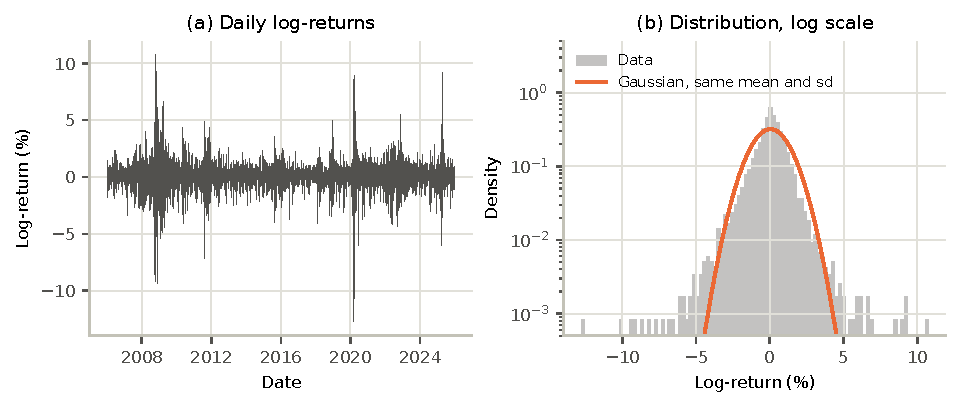
\includegraphics[width=\linewidth]{figures/data_overview.pdf}
  \caption{Daily log-returns of the US market. (a) Over time: calm periods and crises (2008, 2020) alternate. (b) Histogram on a log scale against a Gaussian density with the same mean and standard deviation: the observed tails extend far beyond the Gaussian curve.}
  \label{fig:data}
\end{figure}

%--------------------------------------------------------------------------
\section{Model}\label{sec:model}
%--------------------------------------------------------------------------

\paragraph{Likelihood.} Given $\theta = (\mu, \sigma, \nu)$, the daily returns are independent Student-$t$ variables with location $\mu \in \mathbb{R}$, scale $\sigma > 0$ and $\nu > 2$ degrees of freedom (\cref{fig:dag}):
\begin{equation}\label{eq:likelihood}
  p(r_{1:T} \given \theta) = \prod_{t=1}^T \frac{\Gamma\left(\frac{\nu+1}{2}\right)}{\Gamma\left(\frac{\nu}{2}\right)\sqrt{\nu\pi}\,\sigma}\left[1 + \frac{1}{\nu}\left(\frac{r_t-\mu}{\sigma}\right)^2\right]^{-\frac{\nu+1}{2}}.
\end{equation}
Small $\nu$ means heavy tails, and $\nu \to \infty$ gives the Gaussian; the standard deviation is $\sigma\sqrt{\nu/(\nu-2)}$, not $\sigma$.

\begin{figure}[ht]
  \centering
  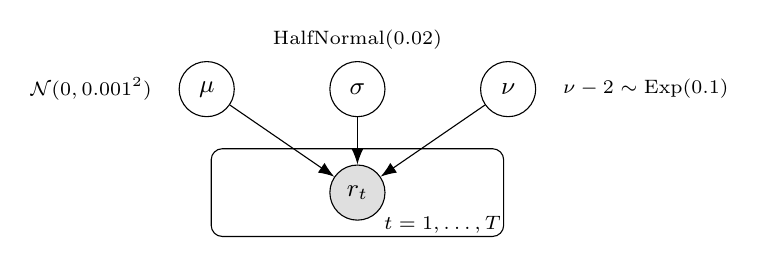
\begin{tikzpicture}[node distance=6mm, every node/.style={font=\small}, inner sep=1pt]
    \node[circle, draw, minimum size=7mm] (mu) {$\mu$};
    \node[circle, draw, minimum size=7mm, right=12mm of mu] (sigma) {$\sigma$};
    \node[circle, draw, minimum size=7mm, right=12mm of sigma] (nu) {$\nu$};
    \node[circle, draw, fill=gray!25, minimum size=7mm, below=6mm of sigma] (r) {$r_t$};
    \node[draw, rounded corners, inner xsep=15mm, inner ysep=2mm, fit=(r), label={[anchor=south east, font=\scriptsize]south east:$t = 1,\dots,T$}] {};
    \draw[-{Latex[length=2mm]}] (mu) -- (r); \draw[-{Latex[length=2mm]}] (sigma) -- (r); \draw[-{Latex[length=2mm]}] (nu) -- (r);
    \node[left=3mm of mu, font=\scriptsize] {$\mathcal{N}(0, 0.001^2)$};
    \node[above=1mm of sigma, font=\scriptsize] {HalfNormal$(0.02)$};
    \node[right=3mm of nu, font=\scriptsize] {$\nu - 2 \sim \mathrm{Exp}(0.1)$};
  \end{tikzpicture}
  \caption{The model as a Bayesian network: white nodes are unknown, the shaded node is observed, the plate repeats it for every day, and the priors are written next to the parameters.}
  \label{fig:dag}
\end{figure}

\paragraph{Priors.} Independent and weakly informative in daily units:
$\mu \sim \mathcal N(0, 0.001^2)$ puts the daily location within $\pm 0.2\%$ (about $\pm 50\%$ a year) with probability 0.95, far wider than what 20 years of data can pin down;
$\sigma \sim \mathrm{HalfNormal}(0.02)$ puts 95\% of its mass below a 4\% daily scale, which covers calm and crisis markets;
$\nu - 2 \sim \mathrm{Exp}(\text{rate } 0.1)$, with mean 10, lets the data choose between very heavy and nearly Gaussian tails, while $\nu > 2$ keeps the variance finite, which the comparison with a Gaussian of matched variance requires. A prior predictive simulation (\cref{tab:prior-predictive}) confirms that these priors are vague but sensible: before seeing any data, they put the 99\% VaR between \val{prior-var99-lo}\% and \val{prior-var99-hi}\% (median \val{prior-var99-med}\%). The posterior is known up to its normalizing constant,
\begin{equation}\label{eq:posterior}
  \pi(\theta\given r_{1:T}) \propto p(r_{1:T}\given\theta)\,\pi(\mu)\,\pi(\sigma)\,\pi(\nu).
\end{equation}
\paragraph{Assumptions.} Days are independent and identically distributed over 20 years, and the tails are symmetric. Independence ignores volatility clustering, so our VaR describes a typical day of the period, not tomorrow.

\paragraph{Risk measures.} For a given $\theta$, VaR and ES have closed forms (derivation in \cref{app:derivations}): with $q = t_\nu^{-1}(\alpha)$ the $\alpha$-quantile and $f_\nu$ the density of the standard Student-$t$,
\begin{equation}\label{eq:var-es}
  \VaR_\alpha(\theta) = -\mu + \sigma q, \qquad
  \ES_\alpha(\theta) = -\mu + \sigma\,\frac{f_\nu(q)}{1-\alpha}\,\frac{\nu+q^2}{\nu-1}.
\end{equation}
Applied to each posterior draw, they give the posterior of VaR and ES. The \emph{predictive} VaR and ES are those of tomorrow's loss under $p(r_{T+1}\given r_{1:T}) = \int p(r_{T+1}\given\theta)\,\pi(\theta\given r_{1:T})\,d\theta$, which folds parameter uncertainty into one number.

\paragraph{Gaussian benchmark.} The Gaussian model $r_t \sim \mathcal N(\mu, s^2)$ has the same prior on $\mu$ and $s \sim \mathrm{HalfNormal}(0.02)$, so the two models differ only in their tails. For each model we report a \emph{plug-in} value at the posterior mean $\bar\theta$, without parameter uncertainty, and the \emph{predictive} value. Comparing the two plug-ins measures the effect of the tails; comparing the Student-$t$ predictive and plug-in values measures the effect of parameter uncertainty.

%--------------------------------------------------------------------------
\section{Method}\label{sec:method}
%--------------------------------------------------------------------------

\paragraph{Sampler.} We sample the posterior on the unconstrained scale $\phi = (\mu, \eta, \lambda)$, with $\sigma = e^\eta$ and $\nu = 2 + e^\lambda$, by random-walk Metropolis--Hastings, so that every proposal is valid \cite{metropolis1953equation,hastings1970monte}. The change of variables adds the Jacobian $|d\sigma/d\eta|\,|d\nu/d\lambda| = \sigma(\nu-2)$ to the target \cite[Prop.~2.1]{leite2026notes}:
\begin{equation}\label{eq:target}
  \log\tilde\pi(\phi) = \log p(r_{1:T}\given\theta) + \log\pi(\mu) + \log\pi(\sigma) + \log\pi(\nu) + \eta + \lambda .
\end{equation}
Algorithm~\ref{alg:mh} is the course's Algorithm~4 with a symmetric Gaussian proposal, so the acceptance probability is a ratio of unnormalized posteriors, computed on the log scale to avoid underflow.

\begin{algorithm}[t]
  \caption{Random-walk Metropolis--Hastings on $\phi$ (one chain of $N$ iterations; $LL^\top$ is the proposal covariance)}
  \label{alg:mh}
  \For{$t = 1, \dots, N$}{
    draw $\varepsilon \sim \mathcal N(0, I_3)$ and $U \sim \mathcal U(0,1)$; set $\phi' = \phi^{(t-1)} + L\varepsilon$\;
    \eIf{$\log U < \log\tilde\pi(\phi') - \log\tilde\pi(\phi^{(t-1)})$}{$\phi^{(t)} \gets \phi'$ \tcp*{accept}}{$\phi^{(t)} \gets \phi^{(t-1)}$ \tcp*{reject: the current value is recorded again}}
  }
\end{algorithm}

\paragraph{Tuning.} Following the course recipe \cite[Sec.~6.5]{leite2026notes}, we start from the posterior mode (MAP, found by BFGS) with the Laplace covariance there: the inverse of minus the Hessian of $\log\tilde\pi$, computed by finite differences, since BFGS's own estimate proved unreliable. \val{cfg-pilot-rounds} pilot runs of \val{cfg-pilot-iter} iterations re-estimate the posterior covariance $\hat\Sigma$ from their own draws, and the proposal $\mathcal N(0, (2.38^2/3)\,\hat\Sigma)$ \cite{roberts1997weak} is then frozen. We run \val{cfg-chains} chains of \val{cfg-n-iter} iterations, started at the MAP plus \val{cfg-start-spread} posterior standard deviations in random directions, and discard a burn-in of \val{cfg-burn-in}, which leaves \val{fit-n-draws} draws. Starting points drawn from the prior proved unsafe: with $\nu$ close to 2, a chain starts on an almost flat ridge of the posterior and needs thousands of iterations to leave it.

\paragraph{Diagnostics and Monte Carlo error.} Each fit must pass three targets: split-$\hat R < 1.01$ \cite{gelman1992inference,vehtari2021rank}, an effective sample size $\mathrm{ESS} = N/\tau \ge 1000$ with $\tau = 1 + 2\sum_k \rho_k$ (summed up to the first negative autocorrelation), and an acceptance rate in $[0.2, 0.5]$. Posterior means are reported with their Monte Carlo standard error $\hat{s}/\sqrt{\mathrm{ESS}}$; quantiles and predictive values with a batch-means error (\val{risk-n-batches} batches per chain, far longer than $\tau$) \cite{flegal2010batch}.

\paragraph{Predictive VaR and ES.} The predictive loss is a mixture over the $N$ posterior draws. Rather than simulating losses, we average exact conditional quantities, a Rao--Blackwellization \cite[Prop.~3.4]{leite2026notes}: the predictive VaR $v$ solves $\frac1N\sum_i \Pr_{\theta_i}(L > v) = 1-\alpha$, and the predictive ES is $\frac{1}{1-\alpha}\frac1N\sum_i \E_{\theta_i}[L\,\mathbf 1\{L > v\}]$, in closed form (\cref{app:derivations}).

\paragraph{Cross-check and implementation.} As an independent check, we also sample the posterior by self-normalized importance sampling, with a Student-$t_4$ proposal centred at the MAP with the Laplace covariance \cite[Ex.~3.4]{leite2026notes}. The samplers, the diagnostics and the risk computations are our own Python code. NumPy, SciPy, pandas and Matplotlib serve only for random numbers, distributions, optimization and plots; we use no probabilistic-programming library.

%--------------------------------------------------------------------------
\section{Validation on simulated data}\label{sec:validation}
%--------------------------------------------------------------------------

\paragraph{Prior only.} With \val{data-n-days} days, the data swamp the prior, so a wrong Jacobian would barely move the posterior. We therefore first run the sampler on the prior alone: its quantiles match the exact prior quantiles within \val{val-prior-dev}\% (\cref{tab:prior-check}).

\paragraph{One simulated data set.} We simulate $T = \val{data-n-days}$ days with $\mu = \val{val-mu-true}\%$, $\sigma = \val{val-sigma-true}\%$ and $\nu = \val{val-nu-true}$, the rounded maximum-likelihood estimate on the real data, where the real posterior lives. All targets are met (\cref{tab:recovery}: $\hat R \le \val{val-rhat-max}$, $\mathrm{ESS} \ge \val{val-ess-min}$, acceptance \val{val-acc-min}), and chains started far apart merge long before the burn-in ends (\cref{fig:validation}). The intervals contain the true $\sigma$ and $\nu$. The interval of $\mu$, [\val{val-mu-lo}, \val{val-mu-hi}]\%, narrowly misses \val{val-mu-true}\%, but the data, not the sampler, are responsible: the maximum-likelihood estimate on these simulated data, \val{val-mu-mle}\%, lies next to our posterior mean of \val{val-mu-mean}\%.

\begin{table}[t]
  \centering
  \caption{Recovery of the true parameters on one simulated data set of the real size, with the diagnostics of the fit. The intervals contain the true $\sigma$ and $\nu$; the narrow miss on $\mu$ comes from the data.}
  \label{tab:recovery}
  \small
  \begin{tabular}{@{}lrrrrrr@{}}
\toprule
Parameter & True & Mean & 95\% interval & $\hat R$ & ESS & MCSE \\
\midrule
$\mu$ & 0.001 & 0.0007507 & [0.0005122, 0.0009928] & 1.0005 & 6,286 & 1.6e-06 \\
$\sigma$ & 0.007 & 0.006906 & [0.006651, 0.007162] & 1.0005 & 6,674 & 1.6e-06 \\
$\nu$ & 2.5 & 2.38 & [2.202, 2.574] & 1.0007 & 7,130 & 1.1e-03 \\
\bottomrule
\end{tabular}

\end{table}

\paragraph{Coverage.} We repeat the whole fit on \val{cov-n-sets} simulated data sets in each of three tail regimes, $\nu \in \{2.5, 4, 8\}$, with lighter settings (chains of \val{cov-cfg-n-iter} iterations). Every coverage, for the parameters and for VaR and ES, lies inside the range expected from a calibrated 95\% interval, \val{cov-band-lo}--\val{cov-band-hi}\% (\cref{tab:coverage}). All \val{cov-converged} fits pass the convergence targets ($\hat R \le \val{cov-rhat-max}$, $\mathrm{ESS} \ge \val{cov-ess-min}$). The standardized errors (truth minus posterior mean, over posterior sd) average between $\val{cov-zmean-min}$ and $\val{cov-zmean-max}$ with sd between \val{cov-zsd-min} and \val{cov-zsd-max}: no material bias, and intervals of the right width. In the $\nu = 4$ regime, coverage sits at the lower edge. This single effect (VaR, ES and $\nu$ miss on the same data sets) reflects a mild upward pull of the prior on $\nu$ (mean standardized error $\val{cov-nu4-z}$).

\begin{table}[t]
  \centering
  \caption{Coverage (\%) of the 95\% posterior intervals over \val{cov-n-sets} simulated data sets per tail regime ($\mu = \val{val-mu-true}\%$, $\sigma = \val{val-sigma-true}\%$, real data size), and the number of fits passing the convergence targets. The last row is the range expected for a calibrated interval (binomial 95\% band).}
  \label{tab:coverage}
  \footnotesize
  \setlength{\tabcolsep}{4pt}
  \begin{tabular}{@{}lrrrrrrrr@{}}
\toprule
Regime & $\mu$ & $\sigma$ & $\nu$ & VaR 99\% & ES 99\% & VaR 99.9\% & ES 99.9\% & Converged fits \\
\midrule
$\nu = 2.5$ & 92 & 95 & 97 & 99 & 99 & 98 & 97 & 100 / 100 \\
$\nu = 4$ & 97 & 94 & 90 & 91 & 90 & 90 & 91 & 100 / 100 \\
$\nu = 8$ & 95 & 94 & 94 & 97 & 96 & 95 & 94 & 100 / 100 \\
Calibrated range & 90--99 & 90--99 & 90--99 & 90--99 & 90--99 & 90--99 & 90--99 &  \\
\bottomrule
\end{tabular}

\end{table}

%--------------------------------------------------------------------------
\section{Results}\label{sec:results}
%--------------------------------------------------------------------------

\subsection{Diagnostics and posterior}

Both models pass every target on the real data (\cref{tab:posterior}; traces in \cref{fig:real-diagnostics}): $\hat R \le \val{fit-rhat-max}$, $\mathrm{ESS} \ge \val{fit-ess-min}$, and acceptance \val{fit-acc-t-min} for the Student-$t$. The tail is very heavy: $\nu = \val{fit-nu}$ [\val{fit-nu-lo}, \val{fit-nu-hi}], close to the maximum-likelihood estimate \val{fit-nu-mle}, and clear of the bound $\nu = 2$. \val{fit-nu-below3} of the \val{fit-n-draws} draws have $\nu < 3$ and all have $\nu < 4$, so the third and fourth moments are infinite. Two consequences matter (\cref{fig:posterior}). First, the standard deviation implied by the Student-$t$, \val{fit-sd}\% [\val{fit-sd-lo}, \val{fit-sd-hi}], is \val{fit-sd-ratio}\% above the sample value (\val{fit-sample-sd}\%): with such tails, the sample standard deviation understates the spread, and the Gaussian model, which reproduces it, is too narrow from the start. Second, the Student-$t$ location (\val{fit-mu}\%), a median-like centre, exceeds the Gaussian mean (\val{fit-g-mu}\%) because of the asymmetry of the data.

\begin{table}[t]
  \centering
  \caption{Posterior summaries and diagnostics on the real data. Implied sd of the Student-$t$: $\sigma\sqrt{\nu/(\nu-2)}$; MCSE: Monte Carlo standard error of the mean.}
  \label{tab:posterior}
  \small
  \begin{tabular}{@{}lrrrrrrr@{}}
\toprule
Model & Quantity & Mean & Sd & 95\% interval & $\hat R$ & ESS & MCSE \\
\midrule
Student-t & $\mu$ (\%) & 0.09665 & 0.012 & [0.07288, 0.1202] & 1.0004 & 6,733 & 0.00015 \\
 & $\sigma$ (\%) & 0.6828 & 0.014 & [0.6558, 0.7102] & 1.0006 & 5,995 & 0.00018 \\
 & $\nu$ & 2.48 & 0.11 & [2.274, 2.708] & 1.0006 & 5,752 & 0.0015 \\
 & Implied sd (\%) & 1.579 & 0.15 & [1.369, 1.921] & 1.0009 & 5,200 & 0.002 \\
Gaussian & $\mu$ (\%) & 0.04083 & 0.017 & [0.007277, 0.07482] & 1.0005 & 9,205 & 0.00018 \\
 & $s$ (\%) & 1.246 & 0.012 & [1.222, 1.271] & 1.0012 & 8,715 & 0.00013 \\
\bottomrule
\end{tabular}

\end{table}

\subsection{Value-at-Risk and Expected Shortfall}

\Cref{tab:risk,fig:risk} answer the question. At 97.5\%, both models give almost the same VaR (\val{VaR97.5-t-pred}\% and \val{VaR97.5-g-pred}\%). From 99\% on they part. The Student-$t$ 99\% VaR is \val{VaR99-t-pred}\% [\val{VaR99-t-lo}, \val{VaR99-t-hi}], \val{VaR99-tails}\% above the Gaussian \val{VaR99-g-pred}\% and equal to the historical value (\val{VaR99-hist}\%). The 99\% ES is \val{ES99-t-pred}\% [\val{ES99-t-lo}, \val{ES99-t-hi}], against \val{ES99-g-pred}\%. At 99.9\%, the Student-$t$ ES is \val{ES99.9-ratio} times the Gaussian one. Parameter uncertainty widens the intervals (the 99.9\% ES lies between \val{ES99.9-t-lo}\% and \val{ES99.9-t-hi}\%) but barely moves the predictive values: by \val{VaR99-param}\% at the 99\% VaR and \val{ES99.9-param}\% at the 99.9\% ES. The tail, not parameter uncertainty, drives the gap. Monte Carlo errors stay below \val{risk-mcse-max} points (\cref{tab:mcse}).

\begin{table}[t]
  \centering
  \caption{One-day VaR and ES (\%) of the US market. Historical: empirical quantile and tail mean of the observed losses. Plug-in: at the posterior mean of the parameters. Predictive: under the posterior predictive distribution. 95\% interval: posterior of $\VaR_\alpha(\theta)$ or $\ES_\alpha(\theta)$.}
  \label{tab:risk}
  \footnotesize
  \setlength{\tabcolsep}{4pt}
  \begin{tabular}{@{}lrrrrrrr@{}}
\toprule
 & & \multicolumn{3}{c}{Gaussian} & \multicolumn{3}{c}{Student-$t$} \\
\cmidrule(lr){3-5}\cmidrule(lr){6-8}
Measure & Historical & Plug-in & Predictive & 95\% interval & Plug-in & Predictive & 95\% interval \\
\midrule
VaR 97.5\% & 2.62 & 2.40 & 2.40 & [2.34, 2.46] & 2.36 & 2.36 & [2.25, 2.48] \\
ES 97.5\% & 4.00 & 2.87 & 2.87 & [2.81, 2.94] & 4.18 & 4.20 & [3.84, 4.64] \\
VaR 99\% & 3.60 & 2.86 & 2.86 & [2.79, 2.93] & 3.59 & 3.60 & [3.36, 3.87] \\
ES 99\% & 5.39 & 3.28 & 3.28 & [3.21, 3.35] & 6.19 & 6.23 & [5.53, 7.07] \\
VaR 99.9\% & 8.09 & 3.81 & 3.81 & [3.73, 3.89] & 9.48 & 9.55 & [8.31, 11.02] \\
ES 99.9\% & 9.70 & 4.16 & 4.16 & [4.07, 4.25] & 16.00 & 16.23 & [13.29, 19.77] \\
\bottomrule
\end{tabular}

\end{table}

\begin{figure}[t]
  \centering
  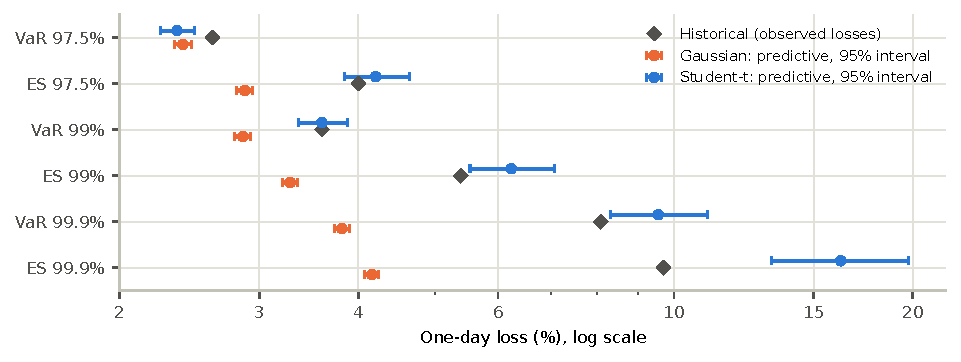
\includegraphics[width=\linewidth]{figures/risk_measures.pdf}
  \caption{Predictive VaR and ES (dots) with the 95\% posterior interval of $\VaR_\alpha(\theta)$ and $\ES_\alpha(\theta)$ (bars), on a log scale, against the historical values (diamonds). The Gaussian model falls short of history; the Student-$t$ matches it at 99\% and exceeds it at 99.9\%.}
  \label{fig:risk}
\end{figure}

\subsection{Model checking}

\Cref{tab:ppc} and \cref{fig:ppc} compare the data with \val{ppc-n-rep} data sets replicated from each posterior \cite{gelman1996posterior}; a $p$-value near 0 or 1 flags a feature the model misses. The Gaussian model fails every tail statistic: it expects almost no day with a loss above 5\%, against \val{ppc-days-loss-obs} observed. The Student-$t$ reproduces the 1\% quantile ($p = \val{ppc-q01-s-p}$) and the number of large losses ($p = \val{ppc-days-loss-s-p}$), but its replicated worst day ranges from $-\val{ppc-worst-t-lo}\%$ to $-\val{ppc-worst-t-hi}\%$, losses never seen, and it misses the mild asymmetry ($p = \val{ppc-asym-s-p}$). Both models fail the volatility-clustering statistic ($p = \val{ppc-acf-s-p}$). The VaR exceedances agree (\cref{tab:exceedances}). At 99\%, the Student-$t$ VaR is beaten on \val{exc99-s} days against \val{exc99-expected} expected, and the Gaussian on \val{exc99-g}. At 99.9\%, the Student-$t$ is conservative (\val{exc99.9-s} against \val{exc99.9-expected}) and the Gaussian is beaten on \val{exc99.9-g} days.

\begin{table}[t]
  \centering
  \caption{Posterior predictive checks: observed statistic, 95\% interval of the statistic over \val{ppc-n-rep} replicated data sets, and $p = \Pr(T(y^{\mathrm{rep}}) \ge T(y) \given y)$. Statistics in \% except the count and the autocorrelation.}
  \label{tab:ppc}
  \footnotesize
  \setlength{\tabcolsep}{4pt}
  \begin{tabular}{@{}lrrrrr@{}}
\toprule
 & & \multicolumn{2}{c}{Gaussian} & \multicolumn{2}{c}{Student-$t$} \\
\cmidrule(lr){3-4}\cmidrule(lr){5-6}
Statistic & Observed & 95\% interval & $p$ & 95\% interval & $p$ \\
\midrule
Worst day (\%) & $-$12.8 & [$-$5.48, $-$3.93] & 1.00 & [$-$79.7, $-$10.4] & 0.10 \\
1\% quantile (\%) & $-$3.6 & [$-$3, $-$2.71] & 1.00 & [$-$4.18, $-$3.12] & 0.55 \\
Days with a loss above 5\% & 21 & [0, 1] & 0.00 & [14, 35] & 0.69 \\
Standard deviation (\%) & 1.25 & [1.21, 1.28] & 0.51 & [1.23, 2.27] & 0.96 \\
1\% + 99\% quantiles (\%) & $-$0.375 & [$-$0.112, 0.274] & 1.00 & [$-$0.458, 0.844] & 0.96 \\
Autocorrelation of |r|, lag 1 & 0.305 & [$-$0.0265, 0.0277] & 0.00 & [$-$0.022, 0.0312] & 0.00 \\
\bottomrule
\end{tabular}

\end{table}

\begin{table}[t]
  \centering
  \caption{In-sample exceedances: number of days whose loss beats the predictive VaR of each model, against the expected number and its binomial 95\% range.}
  \label{tab:exceedances}
  \small
  \begin{tabular}{@{}lrrrr@{}}
\toprule
VaR level & Expected & 95\% range & Gaussian & Student-$t$ \\
\midrule
97.5\% & 126 & 105--148 & 156 & 161 \\
99\% & 50 & 37--65 & 105 & 51 \\
99.9\% & 5 & 1--10 & 46 & 2 \\
\bottomrule
\end{tabular}

\end{table}

\subsection{Sensitivity and cross-check}

Refitting under other reasonable choices (\cref{tab:sensitivity}) shows that the priors do not matter: other priors on $\nu$, $\mu$ (including the one shown at the pitch) and $\sigma$, and the looser bound $\nu > 1$, change $\nu$ and every risk measure by at most \val{sens-prior-maxdev}\%. The data window matters more: on 2016--2025 alone, $\nu = \val{sens-window-nu}$ and the 99\% VaR is \val{sens-window-var99}\% instead of \val{sens-base-var99}\%. Finally, importance sampling with \val{is-n} draws (weight ESS \val{is-ess-pct}\%) reproduces every posterior mean of Metropolis--Hastings within \val{is-max-gap} combined Monte Carlo errors (\cref{tab:crosscheck}).

%--------------------------------------------------------------------------
\section{Discussion and conclusion}\label{sec:discussion}
%--------------------------------------------------------------------------

\paragraph{Answer.} Over 2006--2025, a one-day loss of the US stock market above \val{VaR99-t-pred}\% happens on about 1 trading day in 100; with 95\% probability this threshold lies between \val{VaR99-t-lo}\% and \val{VaR99-t-hi}\%. On those days, the average loss is about \val{ES99-t-pred}\%. A Gaussian model understates them by \val{VaR99-under}\% and \val{ES99-under}\%, and the 99.9\% ES by a factor of \val{ES99.9-ratio}.

\paragraph{Limitations and next steps.} The model assumes independent days, so it gives the risk of an average day of the period, not of tomorrow, and it misses volatility clustering. Pooling calm and crisis periods probably explains the very small $\nu$ and the conservative extrapolation at 99.9\%. The model is also symmetric, depends more on the window than on the priors, and is checked in-sample only. Next steps: a conditional GARCH-$t$ model \cite{bollerslev1986generalized}, a skewed tail, an out-of-sample backtest and simulation-based calibration \cite{talts2018validating}.

%--------------------------------------------------------------------------
%  References (not counted in the 8 pages)
%--------------------------------------------------------------------------

\bibliographystyle{apalike}
\bibliography{references}

%--------------------------------------------------------------------------
%  Appendices (optional, not counted in the 8 pages)
%--------------------------------------------------------------------------
\clearpage
\appendix
\crefalias{section}{appendix}

\section{Derivations}\label{app:derivations}

\paragraph{Jacobian.} With $\sigma = e^\eta$ and $\nu = 2 + e^\lambda$, the density of $\phi$ is $\pi(\theta(\phi))\,|\det J|$ with $|\det J| = e^{\eta} e^{\lambda} = \sigma(\nu-2)$ \cite[Prop.~2.1]{leite2026notes}, which adds $\eta + \lambda$ to the log target \eqref{eq:target}.

\paragraph{Tail expectation of the Student-$t$.} For a standard Student-$t$ variable $Z$ with density $f_\nu$, $f_\nu'(z) = -\frac{(\nu+1)z}{\nu+z^2} f_\nu(z)$, so $\frac{d}{dz}\left[-f_\nu(z)\frac{\nu+z^2}{\nu-1}\right] = z f_\nu(z)$, and for $\nu > 1$
\[
  \E[Z\,\mathbf 1\{Z > c\}] = \int_c^\infty z f_\nu(z)\,dz = f_\nu(c)\,\frac{\nu + c^2}{\nu-1}.
\]
The loss is $L = -\mu + \sigma Z'$ with $Z' = -Z$ also standard Student-$t$. Hence $\Pr(L > v) = \Pr(Z' > c)$ and $\E[L\,\mathbf 1\{L > v\}] = -\mu\Pr(Z' > c) + \sigma\,\E[Z'\,\mathbf 1\{Z' > c\}]$, with $c = (v+\mu)/\sigma$. With $v = \VaR_\alpha(\theta)$, $c = q$ and $\Pr(L > v) = 1-\alpha$, and dividing by $1-\alpha$ gives the ES of \eqref{eq:var-es}. For the Gaussian model, $\E[Z\,\mathbf 1\{Z > c\}] = \varphi(c)$.

\paragraph{Predictive VaR and ES.} The predictive loss is the mixture $\frac1N\sum_i p(L\given\theta_i)$ over the posterior draws. Its exceedance probability $\frac1N\sum_i \Pr_{\theta_i}(L > v)$ is decreasing in $v$, and the predictive VaR is its root at $1-\alpha$. The predictive ES is $\frac{1}{1-\alpha}\frac1N\sum_i \E_{\theta_i}[L\,\mathbf 1\{L > v\}]$, with each term in closed form as above. Averaging these exact conditional quantities instead of simulated losses is a Rao--Blackwellization: it removes the simulation noise of the losses, which matters at 99.9\%, where only one simulated loss in a thousand would fall in the tail.

\section{Additional tables and figures}\label{app:tables}

\begin{table}[h]
  \centering
  \caption{Prior-only check: quantiles of the sampler run without data against the exact prior quantiles ($\mu$ and $\sigma$ in \%). The agreement validates the prior and Jacobian code, which the data would otherwise swamp.}
  \label{tab:prior-check}
  \small
  \begin{tabular}{@{}lrrr@{}}
\toprule
Parameter & Quantile & MH & Exact \\
\midrule
$\mu$ (\%) & 5\% & $-$0.1659 & $-$0.1645 \\
$\mu$ (\%) & 50\% & 0.001021 & 0 \\
$\mu$ (\%) & 95\% & 0.1657 & 0.1645 \\
$\sigma$ (\%) & 5\% & 0.1279 & 0.1254 \\
$\sigma$ (\%) & 50\% & 1.331 & 1.349 \\
$\sigma$ (\%) & 95\% & 3.919 & 3.92 \\
$\nu$ & 5\% & 2.552 & 2.513 \\
$\nu$ & 50\% & 9.103 & 8.931 \\
$\nu$ & 95\% & 31.94 & 31.96 \\
\bottomrule
\end{tabular}

\end{table}

\begin{table}[h]
  \centering
  \caption{Prior predictive check: quantiles of $\nu$, of the daily standard deviation and of the 99\% VaR implied by the prior alone (\val{prior-n-draws} draws).}
  \label{tab:prior-predictive}
  \small
  \begin{tabular}{@{}lrrr@{}}
\toprule
Implied by the prior & 2.5\% & Median & 97.5\% \\
\midrule
$\nu$ & 2.25 & 8.94 & 39 \\
Daily sd (\%) & 0.0752 & 1.66 & 6.69 \\
VaR 99\% (\%) & 0.186 & 4.08 & 15.6 \\
\bottomrule
\end{tabular}

\end{table}

\begin{table}[h]
  \centering
  \caption{Monte Carlo errors (batch means) of the Student-$t$ predictive values and posterior interval endpoints (\%).}
  \label{tab:mcse}
  \small
  \begin{tabular}{@{}lrrrrrr@{}}
\toprule
Measure & Predictive & MCSE & 2.5\% quantile & MCSE & 97.5\% quantile & MCSE \\
\midrule
VaR 97.5\% & 2.362 & 0.001 & 2.251 & 0.001 & 2.483 & 0.002 \\
ES 97.5\% & 4.205 & 0.003 & 3.837 & 0.003 & 4.643 & 0.009 \\
VaR 99\% & 3.597 & 0.002 & 3.358 & 0.002 & 3.870 & 0.005 \\
ES 99\% & 6.234 & 0.005 & 5.531 & 0.006 & 7.072 & 0.018 \\
VaR 99.9\% & 9.551 & 0.010 & 8.306 & 0.011 & 11.016 & 0.031 \\
ES 99.9\% & 16.233 & 0.023 & 13.290 & 0.025 & 19.767 & 0.079 \\
\bottomrule
\end{tabular}

\end{table}

\begin{table}[h]
  \centering
  \caption{Cross-check: posterior means by Metropolis--Hastings and by importance sampling, with their Monte Carlo errors and the gap between them in combined errors.}
  \label{tab:crosscheck}
  \small
  \begin{tabular}{@{}lrrrrr@{}}
\toprule
Quantity & MH mean & MCSE & IS mean & IS error & Gap (in errors) \\
\midrule
$\mu$ (\%) & 0.09665 & 0.0001 & 0.09644 & 6e-05 & 1.4 \\
$\sigma$ (\%) & 0.6828 & 0.0002 & 0.6831 & 7e-05 & 1.5 \\
$\nu$ & 2.48 & 0.001 & 2.481 & 0.0005 & 0.2 \\
VaR 99\% (\%) & 3.598 & 0.002 & 3.599 & 0.0006 & 0.7 \\
ES 99\% (\%) & 6.229 & 0.005 & 6.23 & 0.002 & 0.2 \\
VaR 99.9\% (\%) & 9.544 & 0.009 & 9.546 & 0.003 & 0.2 \\
ES 99.9\% (\%) & 16.17 & 0.02 & 16.17 & 0.008 & 0.0 \\
\bottomrule
\end{tabular}

\end{table}

\begin{figure}[h]
  \centering
  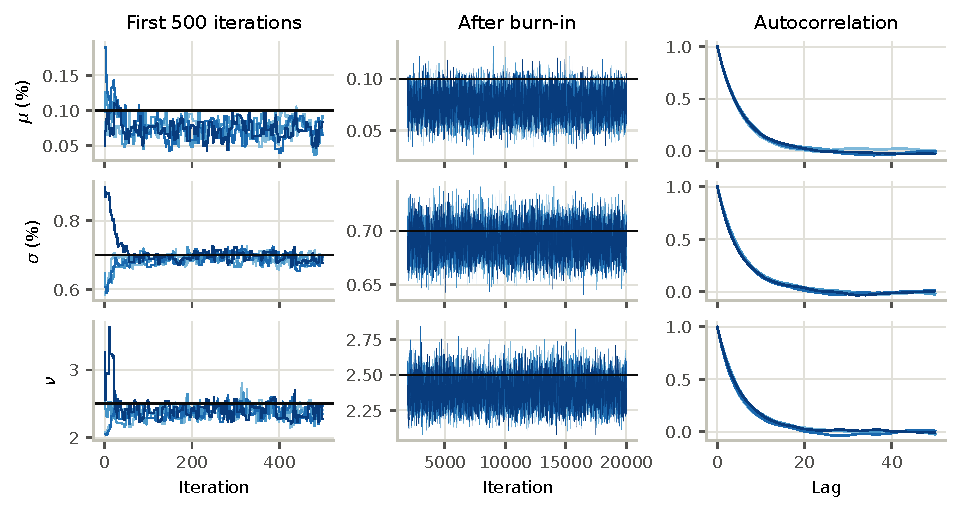
\includegraphics[width=\linewidth]{figures/validation_diagnostics.pdf}
  \caption{Diagnostics of the fit on simulated data (\val{cfg-chains} chains, one shade each; black line: true value). Left: the chains, started far apart, merge within a few hundred iterations. Middle: after burn-in, the traces are stationary and overlap. Right: the autocorrelations decay within a few tens of lags.}
  \label{fig:validation}
\end{figure}

\begin{figure}[h]
  \centering
  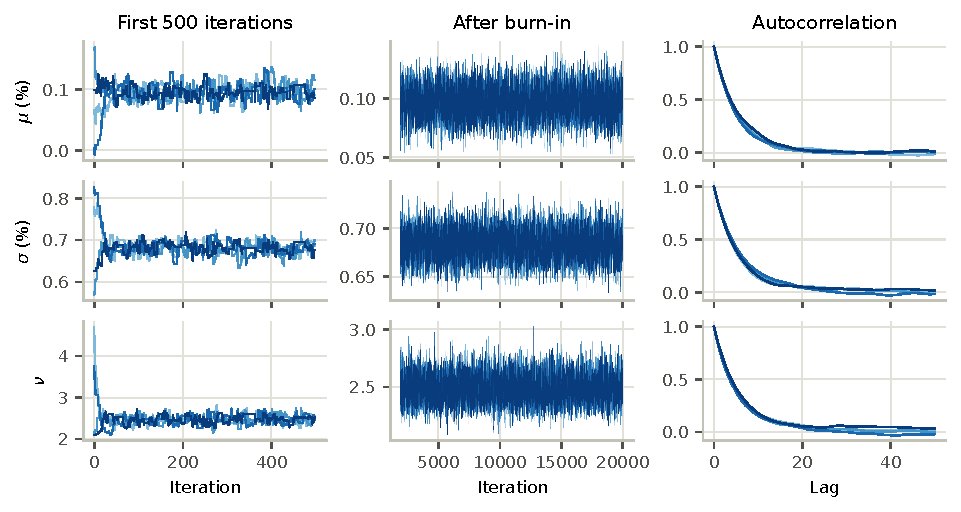
\includegraphics[width=\linewidth]{figures/real_diagnostics.pdf}
  \caption{Diagnostics of the Student-$t$ fit on the real data: first iterations from dispersed starts, traces after burn-in, and autocorrelations (one shade per chain).}
  \label{fig:real-diagnostics}
\end{figure}

\begin{figure}[h]
  \centering
  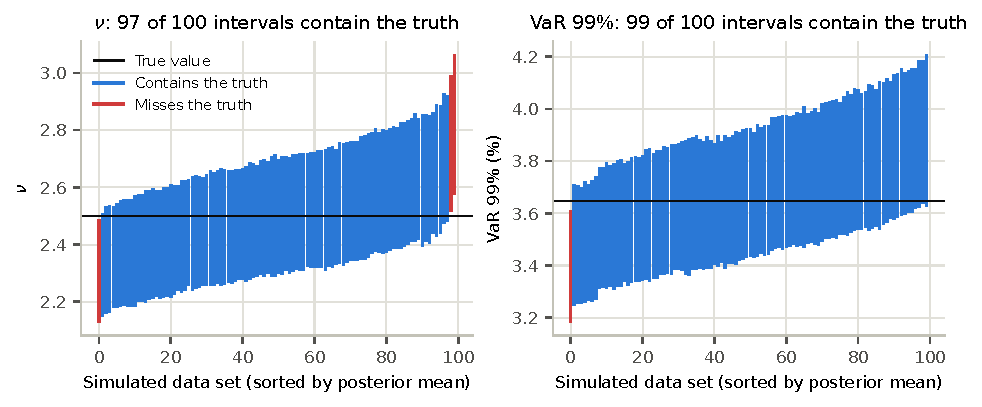
\includegraphics[width=\linewidth]{figures/validation_coverage.pdf}
  \caption{Coverage study, $\nu = 2.5$ regime: the 95\% intervals of $\nu$ and of the 99\% VaR on \val{cov-n-sets} simulated data sets, sorted by posterior mean, against the true value (\val{cov-fig-nu} and \val{cov-fig-var} contain it).}
  \label{fig:coverage}
\end{figure}

\begin{table}[h]
  \centering
  \caption{Summary of the data (returns in \%; the source rounds returns to 0.01\%). The last two rows compare the number of days more than 4 standard deviations from the mean with the number expected under a Gaussian distribution.}
  \label{tab:data}
  \small
  \begin{tabular}{@{}lr@{}}
\toprule
Statistic & Value \\
\midrule
Trading days & 5,031 \\
Period & 03 Jan 2006 -- 31 Dec 2025 \\
Mean (\%) & 0.042 \\
Standard deviation (\%) & 1.246 \\
Worst day (\%) & $-$12.78 \\
Best day (\%) & 10.76 \\
Days beyond 4 sd, observed & 36 \\
Days beyond 4 sd, expected if Gaussian & 0.32 \\
\bottomrule
\end{tabular}

\end{table}

\begin{figure}[h]
  \centering
  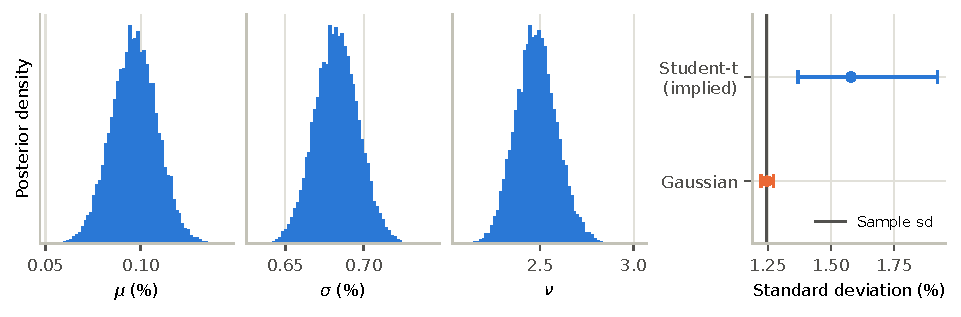
\includegraphics[width=\linewidth]{figures/real_posterior.pdf}
  \caption{Posterior distributions of the Student-$t$ parameters, and the standard deviation of both models (posterior mean and 95\% interval) against the sample standard deviation. The heavy tail ($\nu \approx 2.5$) implies a spread well above the sample standard deviation.}
  \label{fig:posterior}
\end{figure}

\begin{figure}[h]
  \centering
  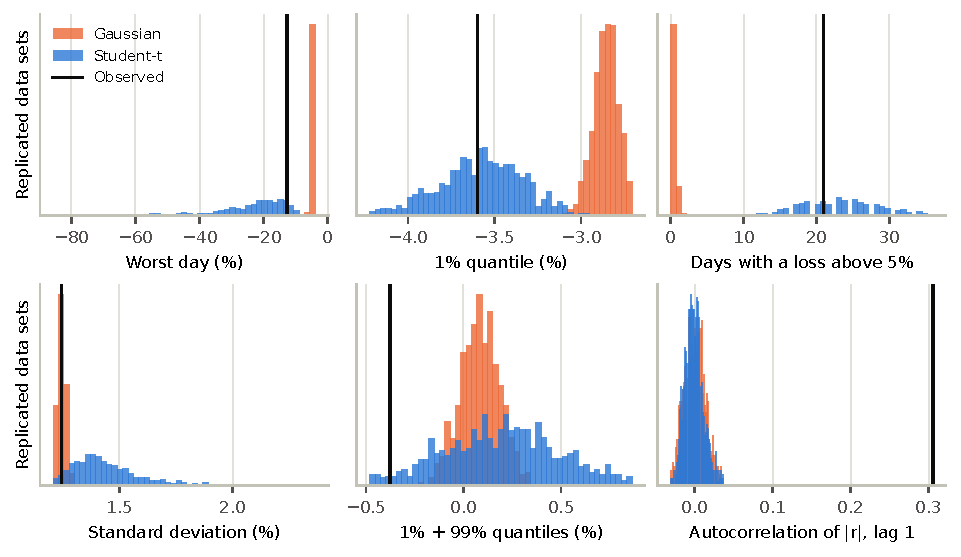
\includegraphics[width=\linewidth]{figures/ppc.pdf}
  \caption{Replicated statistics of both models (histograms; the most extreme 1\% on each side are not drawn) against the observed value (black line). The Gaussian model misses every tail statistic; the Student-$t$ reproduces them; both miss the autocorrelation of $|r_t|$ (volatility clustering).}
  \label{fig:ppc}
\end{figure}


\begin{table}[h]
  \centering
  \caption{Sensitivity of the Student-$t$ results: posterior of $\nu$ and predictive VaR and ES (\%) under each variant. Every refit passes the convergence targets.}
  \label{tab:sensitivity}
  \footnotesize
  \setlength{\tabcolsep}{4pt}
  \begin{tabular}{@{}lrrrrrr@{}}
\toprule
Variant & $\nu$: mean [95\% interval] & VaR 99\% & ES 99\% & VaR 99.9\% & ES 99.9\% & max $\hat R$ \\
\midrule
Baseline & 2.48 [2.27, 2.71] & 3.60 & 6.23 & 9.55 & 16.23 & -- \\
$\nu$ prior rate 0.05 & 2.48 [2.27, 2.70] & 3.60 & 6.23 & 9.54 & 16.21 & 1.0010 \\
$\nu$ prior rate 0.5 & 2.47 [2.27, 2.69] & 3.60 & 6.26 & 9.60 & 16.34 & 1.0005 \\
$\mu$ prior sd 0.01 (pitch) & 2.48 [2.27, 2.70] & 3.60 & 6.24 & 9.57 & 16.27 & 1.0007 \\
$\sigma$ prior scale 0.05 & 2.48 [2.28, 2.71] & 3.59 & 6.22 & 9.53 & 16.18 & 1.0007 \\
$\nu > 1$ instead of $\nu > 2$ & 2.48 [2.27, 2.70] & 3.60 & 6.25 & 9.57 & 16.29 & 1.0006 \\
Window 2016--2025 & 2.67 [2.34, 3.04] & 3.26 & 5.43 & 8.20 & 13.41 & 1.0004 \\
\bottomrule
\end{tabular}

\end{table}

\clearpage
\section{Code}\label{app:code}

The code is in \texttt{code/}; \texttt{code/README.md} lists which script produces each table, figure and number of this report. All settings are in \texttt{code/config.toml}; the reusable functions are in \texttt{code/src/}: the model and priors (\texttt{model.py}), the sampler and its tuning (\texttt{mh.py}), the diagnostics (\texttt{diagnostics.py}), and VaR and ES (\texttt{risk.py}). The nine scripts in \texttt{code/scripts/} run in order and take about eight minutes in total.

\end{document}
